\documentclass[aps,prl,floatfix,twocolumn,footinbib,superscriptaddress]{revtex4-1}
\usepackage{epsfig}
\usepackage{float}
\usepackage{epstopdf} %converting to PDF
\usepackage{braket}
\usepackage[utf8]{inputenc}
\usepackage{amsmath}
\usepackage{amssymb}
\usepackage{esint}
\usepackage{xcolor}
\usepackage{bbm}


\begin{document}
\title{Revealing the emergence of the classicality in nitrogen-vacancy centers}

%Alt titles: 
%\title{Revealing the emergence of the classicality via NV center measurements}
%Revealing the emergence of the classical world via NV center measurements
%The emergence of a classical NV-center spin /via nuclear-spin decoherence
%The emergence of redundancy in nuclear spin environments of an NV center.
%Quantum Darwinism in action (in the lab): The emergence of redundancy in nuclear spin environments of an NV center.

\global\long\def\avg#1{\langle#1\rangle}

\global\long\def\p{\prime}

\global\long\def\dg{\dagger}

\global\long\def\ket#1{|#1\rangle}

\global\long\def\bra#1{\langle#1|}

\global\long\def\proj#1#2{|#1\rangle\langle#2|}

\global\long\def\inner#1#2{\langle#1|#2\rangle}

\global\long\def\tr{\mathrm{tr}}

\global\long\def\pd#1#2{\frac{\partial#1}{\partial#2}}

\global\long\def\spd#1#2{\frac{\partial^{2}#1}{\partial#2^{2}}}

\global\long\def\der#1#2{\frac{d#1}{d#2}}

\global\long\def\im{\imath}

\global\long\def\S{\mathcal{S}}

\global\long\def\A{\mathcal{A}}

\global\long\def\F{\mathcal{F}}

\global\long\def\E{\mathcal{E}}

\global\long\def\As{{^{\sharp}}\hspace{-1mm}\mathcal{A}}

\global\long\def\Fs{{^{\sharp}}\hspace{-0.7mm}\mathcal{F}}

\global\long\def\Es{{^{\sharp}}\hspace{-0.5mm}\mathcal{E}}

\global\long\def\EsG{{^{\sharp}}\hspace{-0.5mm}\mathcal{E}_{G}}

\global\long\def\EsB{{^{\sharp}}\hspace{-0.5mm}\mathcal{E}_{B}}

\global\long\def\FsG{{^{\sharp}}\hspace{-0.5mm}\F_{G}}

\global\long\def\FsB{{^{\sharp}}\hspace{-0.5mm}\F_{B}}

\global\long\def\Fd{{^{\sharp}}\hspace{-0.7mm}\mathcal{F}_{\delta}}

\global\long\def\EG{\mathcal{E}_{G}}

\global\long\def\EB{\mathcal{E}_{B}}

\global\long\def\O{\mathcal{O}}

\global\long\def\SgF{\S d\F}

\global\long\def\SgEF{\S d\left(\E/\F\right)}

\global\long\def\U{\mathcal{U}}

\global\long\def\V{\mathcal{V}}

\global\long\def\H{\mathbf{H}}

\global\long\def\SO{\Pi_{\S}}

\global\long\def\PO{\hat{\Pi}_{\S}}

\global\long\def\SSH{\tilde{\Pi}_{\S}}

\global\long\def\EO{\Upsilon_{k}}

\global\long\def\ESH{\Omega_{k}}

\global\long\def\HSF{\mathbf{H}_{\S\F}}

\global\long\def\HSEF{\mathbf{H}_{\S\E/\F}}

\global\long\def\HS{\mathbf{H}_{\S}}

\global\long\def\ES{H_{\S}(t)}

\global\long\def\ESo{H_{\S}(0)}

\global\long\def\EgF{H_{\SgF} (t)}

\global\long\def\EgE{H_{\S d\E}(t)}

\global\long\def\EgEF{H_{\SgEF} (t)}

\global\long\def\EF{H_{\F}(t)}

\global\long\def\EFo{H_{\F}(0)}

\global\long\def\ESF{H_{\S\F}(t)}

\global\long\def\ESEF{H_{\S\E/\F}(t)}

\global\long\def\ESSEF{H_{\tilde{\S}\S\E/\F}(t)}

\global\long\def\EEFo{H_{\E/\F}(0)}

\global\long\def\EEF{H_{\E/\F}(t)}

\global\long\def\HPB{H(\PB)}

\global\long\def\MI{I\left(\S:\F\right)}

\global\long\def\aMI{\left\langle \MI\right\rangle _{\Fs}}

\global\long\def\BS{\Pi_{\S} }

\global\long\def\PB{\hat{\Pi}_{\S} }

\global\long\def\QD{\mathcal{D}\left(\Pi_{\S}:\F\right)}
\global\long\def\QD{\mathcal{D}(\Pi_{\S}:\F)}

\global\long\def\QDp{\mathcal{D}\left(\PB:\F\right)}
\global\long\def\QDpIL{\mathcal{D}(\PB:\F)}

\global\long\def\JI{J\left(\Pi_{\S}:\F\right)}

\global\long\def\CI{H\left(\F\left|\Pi_{\S}\right.\right)}

\global\long\def\CIp{H\left(\F\left|\PB\right.\right)}

\global\long\def\CS{\rho_{\F\left|s\right.}}

\global\long\def\CSu{\tilde{\rho}_{\F\left|s\right.}}

\global\long\def\CSp{\rho_{\F\left|\hat{s}\right.}}

\global\long\def\CEF{H_{\F\left|s\right.}}

\global\long\def\CEFp{H_{\F\left|\hat{s}\right.}}

\global\long\def\psiz{\ket{\psi_{\E\left|0\right.\hspace{-0.4mm}}}}

\global\long\def\psio{\ket{\psi_{\E\left|1\right.\hspace{-0.4mm}}}}

\global\long\def\psiinner{\inner{\psi_{\E\left|0\right.\hspace{-0.4mm}}}{\psi_{\E\left|1\right.\hspace{-0.4mm}}}}

\global\long\def\QDz{\boldsymbol{\delta}\left(\S:\F\right)_{\left\{  \sigma_{\S}^{z}\right\}  }}

\global\long\def\NQD{\bar{\boldsymbol{\delta}}\left(\S:\F\right)_{\BS}}

\global\long\def\EFS{H_{\F\left| \BS\right. }(t)}

\global\long\def\EFSM{H_{\F\left| \left\{  \ket m\right\}  \right. }(t)}

\global\long\def\Hol{\chi\left(\Pi_{\S}:\F\right)}
\global\long\def\HolIL{\chi(\Pi_{\S}:\F)}

\global\long\def\Holp{\chi\left(\PB:\F\right)}
\global\long\def\HolpIL{\chi(\PB:\F)}

\global\long\def\ch{\raisebox{0.5ex}{\mbox{\ensuremath{\chi}}}_{\mathrm{Pointer}}}

\global\long\def\rhoS{\rho_{\S}(t)}

\global\long\def\rhoSo{\rho_{\S}(0)}

\global\long\def\rhoSF{\rho_{\S\F} (t)}

\global\long\def\rhoSgEF{\rho_{\SgEF} (t)}

\global\long\def\rhoSgF{\rho_{\SgF} (t)}

\global\long\def\rhoF{\rho_{\F}(t)}

\global\long\def\rhoFp{\rho_{\F}(\pi/2)}

\global\long\def\LE{\Lambda_{\E}(t)}

\global\long\def\LEc{\Lambda_{\E}^{\star}(t)}

\global\long\def\LEij{\Lambda_{\E}^{ij}(t)}

\global\long\def\LF{\Lambda_{\F}(t)}

\global\long\def\LFij{\Lambda_{\F}^{ij} (t)}

\global\long\def\LFc{\Lambda_{\F}^{\star}(t)}

\global\long\def\LEF{\Lambda_{\E/\F} (t)}

\global\long\def\LEFij{\Lambda_{\E/\F}^{ij}(t)}

\global\long\def\LEFc{\Lambda_{\E/\F}^{\star}(t)}

\global\long\def\Lkij{\Lambda_{k}^{ij}(t)}

\global\long\def\Hb{H}

\global\long\def\kE{\kappa_{\E}(t)}

\global\long\def\kEF{\kappa_{\E/\F}(t)}

\global\long\def\kF{\kappa_{\F}(t)}

\global\long\def\ts{t=\pi/2}

\global\long\def\QCB{\bar{\xi}_{QCB}}

\global\long\def\mc#1{\mathcal{#1}}

\global\long\def\MD{\lambda}

\global\long\def\up{\mathord{\uparrow}}

\global\long\def\down{\mathord{\downarrow}}

\global\long\def\Cku{\rho_{k\left|\up\right.}}

\global\long\def\Ckd{\rho_{k\left|\down\right.}}

\global\long\def\f{\mathcal{J}}

\global\long\def\onlinecite#1{\cite{#1}}

\newcommand{\todo}[1]{\textcolor{red}{#1}}

\title{Supplementary Information -- Revealing the emergence of the classicality in nitrogen-vacancy centers}

\author{T. Unden}
\affiliation{Institute for Quantum Optics, Ulm University, Albert-Einstein-Allee 11, Ulm 89081, Germany}

\author{D. Louzon}
\affiliation{Institute for Quantum Optics, Ulm University, Albert-Einstein-Allee 11, Ulm 89081, Germany}
\affiliation{Racah Institute of Physics, The Hebrew University of Jerusalem, Jerusalem 91904, Israel}

\author{M. Zwolak}
\affiliation{Center for Nanoscale Science and Technology, National Institute of Standards and Technology, Gaithersburg,
Maryland 20899, U.S.A.}

\author{W. H. Zurek}
\affiliation{Theory Division, Los Alamos National Laboratory, Los Alamos, NM, 87545, U.S.A.}

\author{F. Jelezko}
\affiliation{Institute for Quantum Optics, Ulm University, Albert-Einstein-Allee 11, Ulm 89081, Germany}
\affiliation{Center for Integrated Quantum Science and Technology (IQ$^\text{{st}}$), Ulm University, 89081 Germany}

\maketitle

\renewcommand\thefigure{S\arabic{figure}}

\section{Control}

In Fig.~\ref{fig:S1}, we show the coherent interaction between the electron and nuclear spin $\E_1$ for two different strengths of the filter-function. When the effective coupling increases from $\frac{0.1\cdot A_\perp}{2}$ to $\frac{0.2\cdot A_\perp}{2}$, the frequency of the oscillations doubles. Figure~\ref{fig:S2} shows the the coherent interaction between the electron and nuclear spin $\E_1$ for a fixed AXY repetition number and increasing effective coupling for the cases $N=8,16,32$. We use a filter strength of about $0.2\cdot A_\perp$. For a certain $N$, we fine-tune $f_{DD}$ to achieve two qubit $\pi/2$-rotations.

\begin{figure}[h]
\centerline{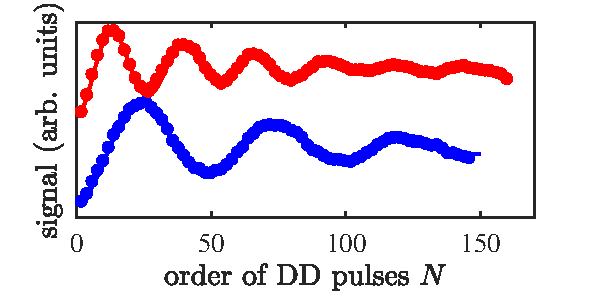
\psfig{file=figure/SFig1.pdf, width=1\linewidth}}
\caption{Electron spin coherence versus the DD pulse number when the pulse spacing is adjusted to the resonance of carbon spin 1. The entangling operation is via the AXY pulse sequence with effective coupling strength $f_{DD}=0.1$ (blue) and doubled strength $2f_{DD}$ (red) with parameters given by the DD filter function equations, Eq. (8) in the Methods section of the main text. Solid lines are the result of a simulation, assuming dephasing and the measured hyperfine coupling strength (see Table 1). Errors are smaller than the data points.}
\label{fig:S1}
\end{figure}

\begin{figure}[h]
\centerline{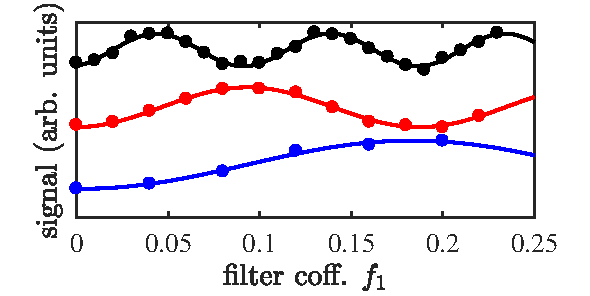
\psfig{file=figure/SFig2.pdf, width=1\linewidth}}
\caption{Electron spin coherence versus the effective coupling. The entangling operation is via AXY-8 (blue)/16 (red)/32 (black). The solid lines are cosine fits (SSE of $4\cdot10^{-4}$, $6\cdot10^{-4}$ and $29\cdot10^{-4}$ ). Errors are smaller than the data points.}
\label{fig:S2}
\end{figure}

\section{Hyperfine coupling strength}

Table~\ref{tab:HF} shows the hyperfine coupling strength of the different nuclei. The parallel component is estimated by analysis of AXY spectra and the perpendicular component by analyzing oscillations (see Fig.~\ref{fig:S1}) caused by resonant interaction when interaction time is increased. 

\begin{table}
\caption{Hyperfine interaction strength of the register.}
\begin{center}
\begin{tabular}{ c c c }
  \hline
  \textbf{nuc. spin} & \textbf{$\frac{A_\parallel}{2\pi}$ (kHz)} & \textbf{$\left| \frac{A_\perp}{2\pi}\right|$ (kHz)} \\ 
  \hline
  1 & $\phantom{-}93.5$ & $45.8$ \\
  2 & $\phantom{-}49.5$ & $35.3$ \\
  3 & $-26.3$ &$22.0$\\
  4 & $-47.1$ & $42.5$\\
  \hline
\end{tabular}
\end{center}
\label{tab:HF}
\end{table}

\section{NV Ramsey}

A Ramsay ($\frac{\pi}{2}$-pulse - wait $\tau$ - $\frac{\pi}{2}$-pulse) experiment performed on the electronic spin of NV center is shown in Fig.~\ref{fig:S3}. The four strongest coupled nuclear spins are polarized into the $\ket{+x}$-state in this measurement. The initial state is therefore in accordance with the initial state of the experiment shown in the second part of results section (see main text). 

\begin{figure}
\centerline{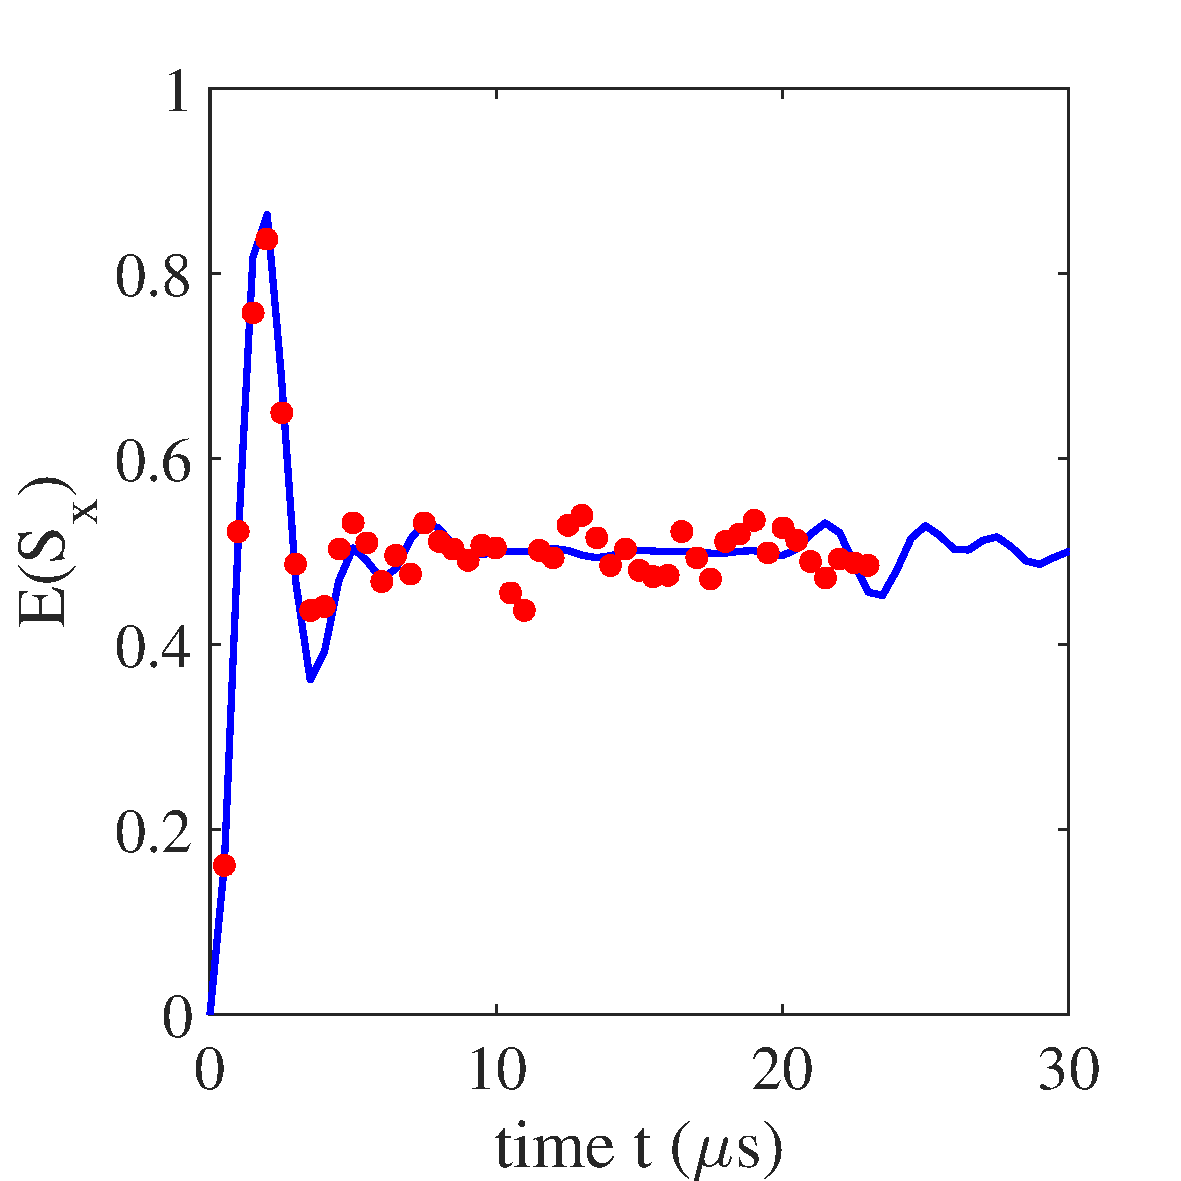
\psfig{file=figure/SFig3.pdf, width=0.7\linewidth}}
\caption{NV Ramsay experiment when the nuclear spin register is polarized to the $\ket{+_x}$ state. Solid line corresponds to a simulation based on the measured hyperfine interactions. Errors are smaller than the data points.}
\label{fig:S3}
\end{figure}

\section{Multiple quantum coherence}

In Fig.~\ref{fig:S4}a, we show our sequence for testing quantum correlations after creating the redundant state. It is based on a Loschmidt echo, where the echo is perturbed by a free evolution period in between both entangling gates ($\pm R_x(\frac{\pi}{2})$). By increasing the free evolution period $\tau$, oscillations, Fig.~\ref{fig:S4}b, get visible, which can be attributed to the Larmor precession (about $0.5$ MHz) of the three nuclear spins and the sum of all Larmor frequencies (about $1.5$ MHz), which is a hint for multiple quantum coherences. The free evolution period was composed of a CPMG sequence, where the pulse spacing did not match to nuclear spin transitions. The reconstructed density matrix (shown in Fig.~\ref{fig:S4}c) is the result of a comparison of experimental data with simulated data (that takes only the diagonal and outer off-diagonal entries of the density matrix into account) and yields a state fidelity of $40$ \% with respect to a fully entangled GHZ state. 

\begin{figure}
\centerline{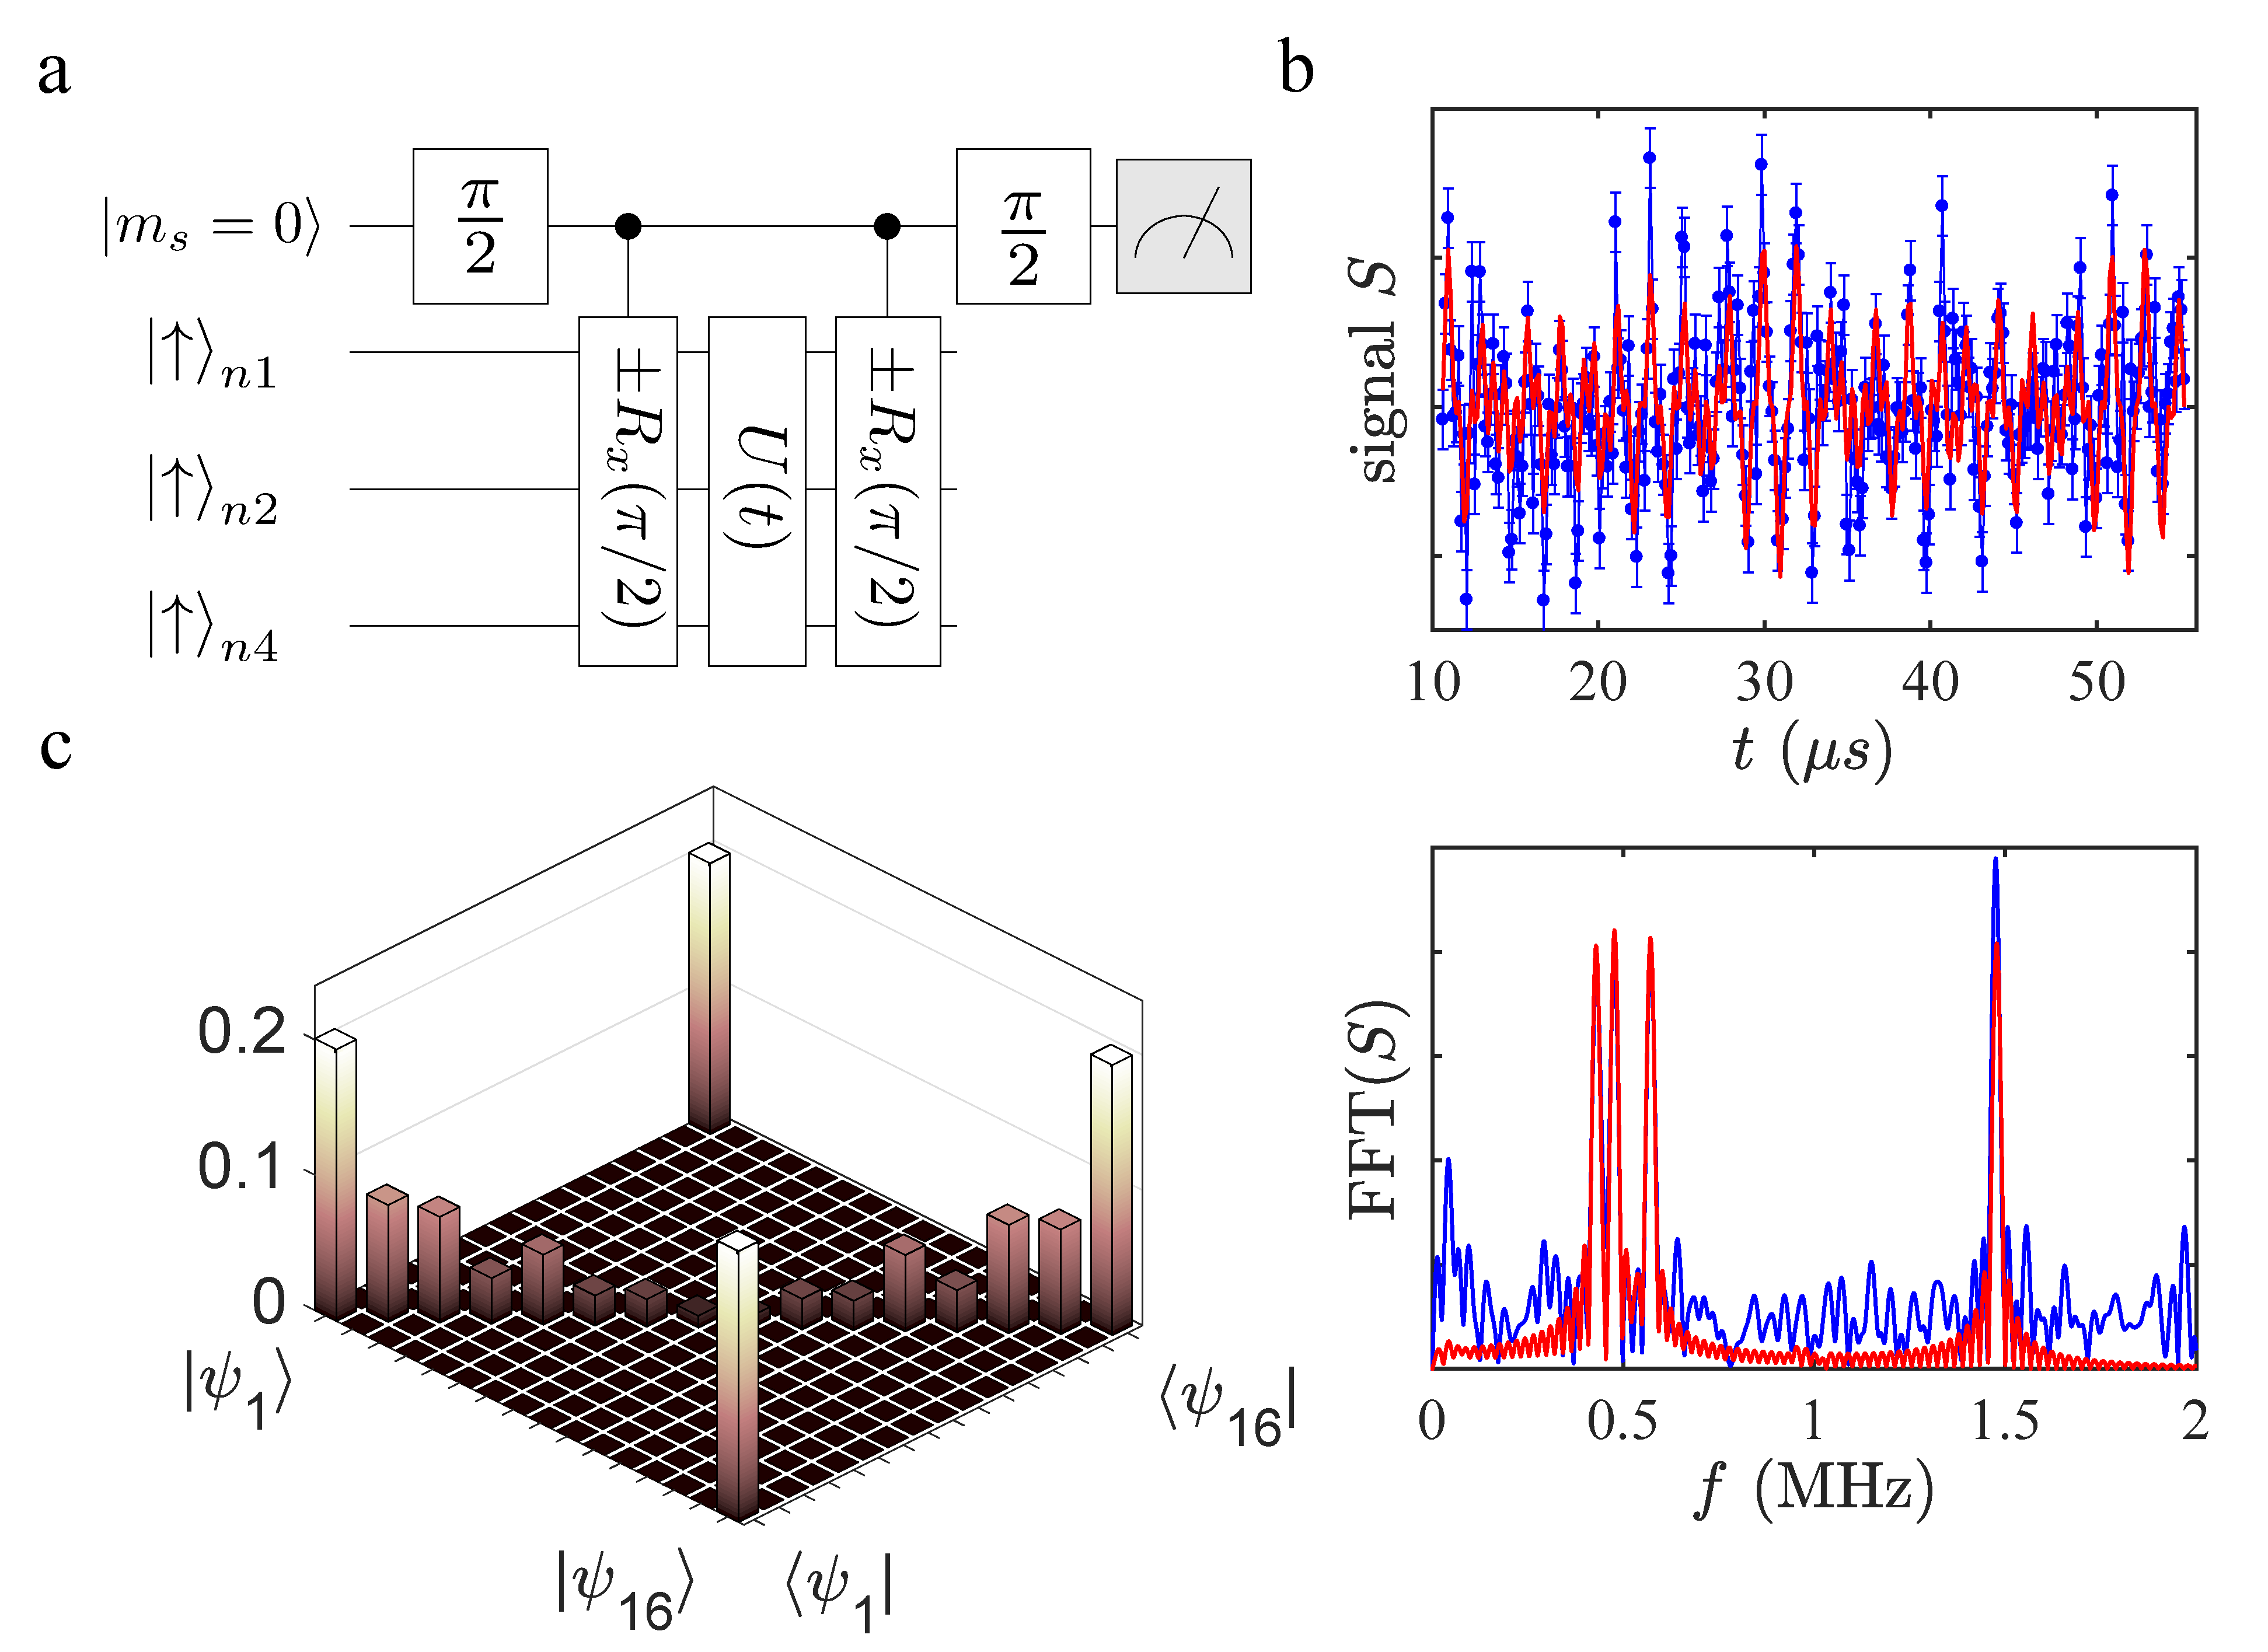
\psfig{file=figure/SFig4.pdf, width=1\linewidth}}
\caption{Results of the Loschmidt echo. (a) Sequence for testing multiple coherences present in the system. (b) Measurement (blue) and simulation (red) results with corresponding Fast Fourier Transform (FFT). Single Larmor frequency at a magnetic field of about $440G\approx 0.5 MHz$ is visible. Shift of each nuclear spin precession is due hyperfine interaction. Also visible is the sum of individual Larmor frequencies, which indicate multiple coherences present in the system. Error bars represent one standard deviation. (c) Reconstructed density matrix. With $\ket{\psi_1}=\ket{\uparrow}\ket{+}\ket{+}\ket{+}\ket{+}$ and  $\ket{\psi_{16}}=\ket{\downarrow}\ket{-}\ket{-}\ket{-}\ket{-}$.}
\label{fig:S4}
\end{figure}

\section{Chernoff Information}

In Fig.~\ref{fig:S5}, we show the quantum Chernoff information~\cite{Audenaert07} averaged over the four nuclear spins~\cite{Zwolak14,zwolak16}, i.e., the typical quantum Chernoff information $\QCB$, which sets an upper bound for redundancy rate in the asymptotic (large fragment size) limit. The redundancy is given by $\QCB \Es / \ln 1/\delta$, where $\Es$ is the total number of components in the environment. This equation requires sufficiently precise information (i.e., a small information deficit $\delta$) in order for the asymptotic limit to be accurate, otherwise the redundancy would be incorrectly given a value greater than $\Es$. 

\begin{figure}
\centerline{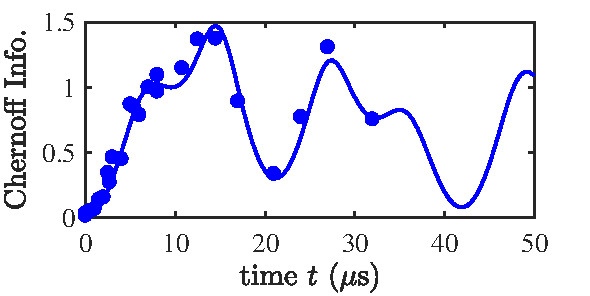
\psfig{file=figure/SFig5.pdf, width=1\linewidth}}
\caption{Chernoff Information. Solid line corresponds to a simulation based on the measured hyperfine interactions. Errors are smaller than the data points.}
\label{fig:S5}
\end{figure}

\section{Potential redundancy in $^{13}C$ enriched diamonds}

Based on recently published hyperfine data of a 510 nuclear spin cluster~\cite{Nizovtsev18}, we show in Fig.~\ref{fig:S6} the number of central spin records over interaction time. The amount of information is estimated using quantum Chernoff information~\cite{Zwolak14,zwolak16}. The results are averaged over ten different realizations of the specified settings. In a highly concentrated $^{13}C$-diamond, a large amount (hundreds) of central spin records could be observed within a timescale of $\mu s$ when the initial nuclear spin polarization is large (see, e.g., Ref.~\cite{Parker18}). At  high $^{13}C$ concentration unwanted  interaction (here in our analysis neglected) between nuclear spins will appear, but our current results show, that on the timescale ($\approx \mu s$) where redundancy increases, these interactions ($\approx$ Hz - kHz) can be neglected for a moderate $^{13}C$ enrichment and a high initial nuclear spin polarization.

\begin{figure}
\centerline{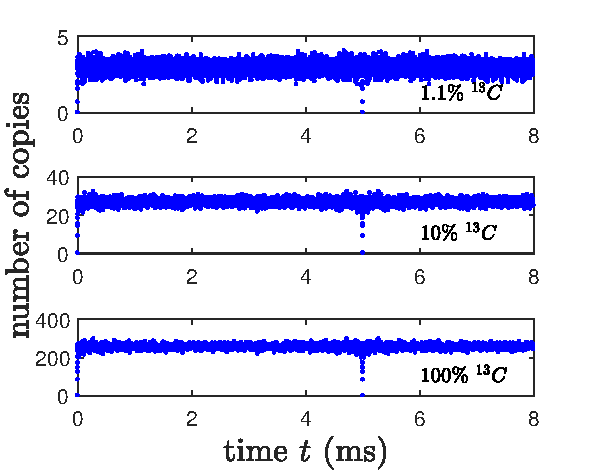
\psfig{file=figure/SFig6.pdf, width=1\linewidth}}
\caption{Number of copies of information versus the interaction time for various $^{13}C$ concentrations.}
\label{fig:S6}
\end{figure}


\bibliographystyle{apsrev}
\bibliography{reference}

\end{document}



